\documentclass[10pt, a4paper]{scrartcl}

\usepackage{vorschule}
\usepackage[
	typ=ab,
	fach=Mathematik,
	lerngruppe={Jg.7},
	nummer=1,
	module={Symbole,Lizenzen},
	seitenzahlen=keine,
	farbig,
	lizenz=cc-by-nc-sa-4,
]{schule}

\usepackage[
	kuerzel=Ngb,
	reihe={Ganze Zahlen},
	version={2020-08-11},
]{ngbschule}

\author{J. Neugebauer}
\title{Hin und her}
\date{\Heute}

\setzeAufgabentemplate{ngbnormal}


\begin{document}
\ReiheTitel

\begin{aufgabe}
	Setzt euch mit zwei Personen zusammen. Schlagt im Buch Seite 6 auf und lest die Spielregeln des Spiels \enquote{Hin und her}.
	
	Bastelt dann die nötigen Materialien:
	
	\begin{itemize}
		\item Als Spielfiguren könnt ihr zum Beispiel Papierschnipsel mit Symbolen drauf oder Geldmünzen nehmen.
		\item Für die Würfel könnt ihr ein A4 Blatt dreimal in der Mitte falten und anschließend an den Faltkanten zerschneiden. Auf sechs der Karteikarten schreibt ihr die Zahlen Eins bis Sechs. Und auf den verbleibenden beiden die Symbole \enquote{+} und \enquote{-}. Legt die Karten verdeckt auf den Tisch und zieht zum Würfeln jeweils eine Zahl und ein Symbol.
	\end{itemize}
	
	Spielt dann zwei Runden des Spiels.
\end{aufgabe}

\begin{aufgabe}
	Die Spielzüge eurer Figuren kann man auch als Rechnung aufschreiben. Steht eure Figur zum Beispiel auf dem Feld mit der \enquote{4} und ihr zieht ein \enquote{-} und die Zahl \enquote{5}, dann lautet die Rechnung:
	
	\[ 4 - 5 = -1 \]
	
	Überlegt euch \textbf{für jedes der folgenden Beispiele drei unterschiedliche Spielsituationen} und die dazugehörigen Rechenterme. (\emph{Für fehlende Informationen könnt ihr euch selber Zahlen aussuchen.})
	
	\begin{enumerate}
		\item Die Figur steht im positiven Bereich und es wird \enquote{-} gezogen.
		\item Die Figur steht im negativen Bereich und es wird \enquote{+} gezogen.
		\item Die Figur steht im positiven oder negativen Bereich und zieht auf das Startfeld mit der \enquote{0}.
		\item Die Figur steht im positiven oder negativen Bereich und wird beim Zug über das Startfeld mit der \enquote{0} bewegt.
	\end{enumerate}
\end{aufgabe}

\begin{aufgabe}[subtitle=Hausaufgabe]
	Lest im Buch Seite 8 und 9 und bearbeitet auf Seite 164 Aufgaben 1-3.
\end{aufgabe}

\newpage

\begin{center}
	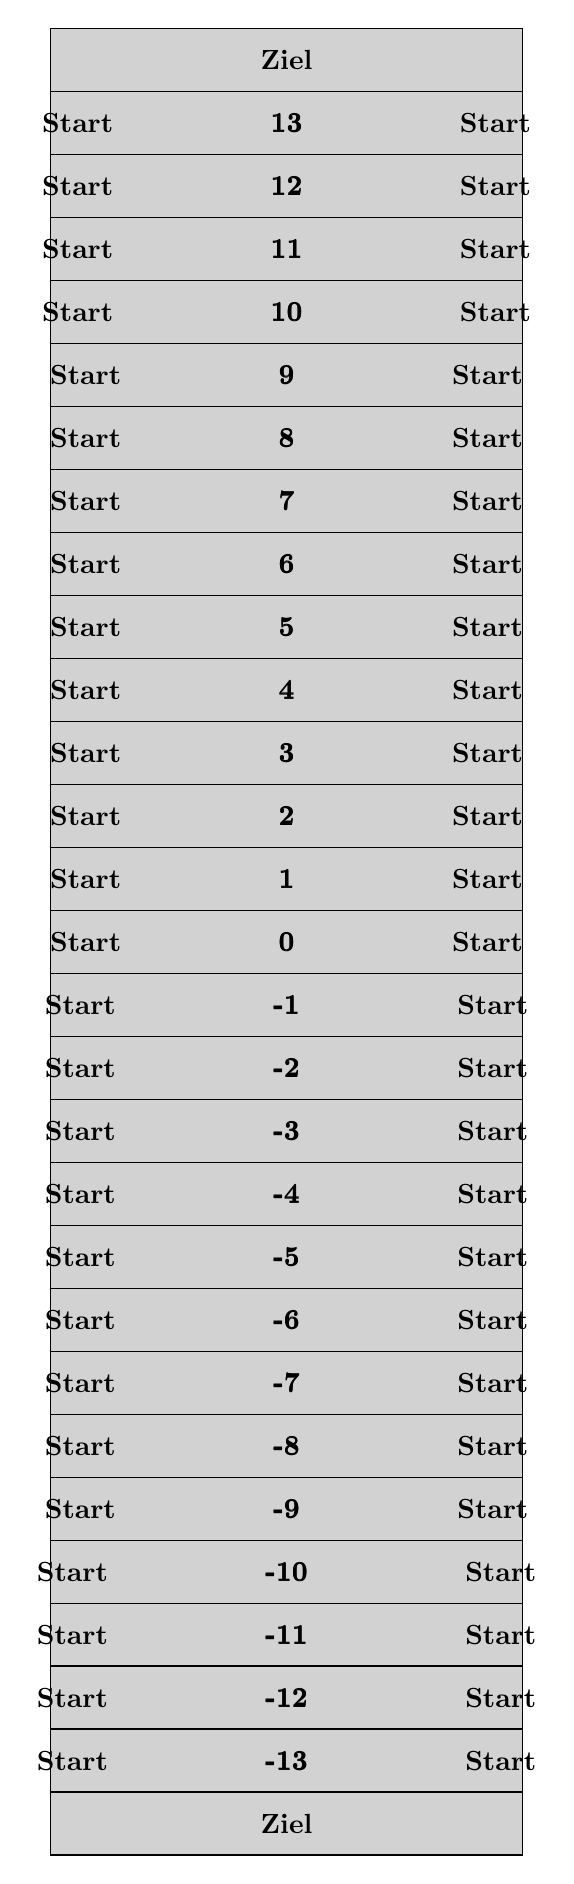
\begin{tikzpicture}[scale=1,font={\bfseries}]
		\pgfmathsetmacro \vSize {0.8}
	\draw[fill=gray!35] (0,0) rectangle +(6,\vSize) node[pos=.5] {Ziel};
	\foreach \i in {13,...,-13} {%
		\ifthenelse{\equal{\i}{0}}{%
			\draw[fill=gray!35] (0,{(13-\i+1)*-1*\vSize}) rectangle +(6,\vSize) node[pos=.5] {Start\hspace{2cm}\i\hspace{2cm}Start};
		}{%
			\draw[] (0,{(13-\i+1)*-1*\vSize}) rectangle +(6,\vSize) node[pos=.5] {\i};
		}%
	}
	\draw[fill=gray!35] (0,{28*-1*\vSize}) rectangle +(6,\vSize) node[pos=.5] {Ziel};
	\end{tikzpicture}
\end{center}

\end{document}
